% ============================================================================
%  All figure environments in one place. Chapters call \figMcCrossover, etc.
%  Conceptual diagrams are drawn in TikZ. Plot files in figures/ are regenerated
%  by scripts/make_thesis_figures.py and found via \graphicspath in preamble.tex.
% ============================================================================

\newcommand{\figPanelBalance}{%
  \begin{figure}[htb]
    \centering
    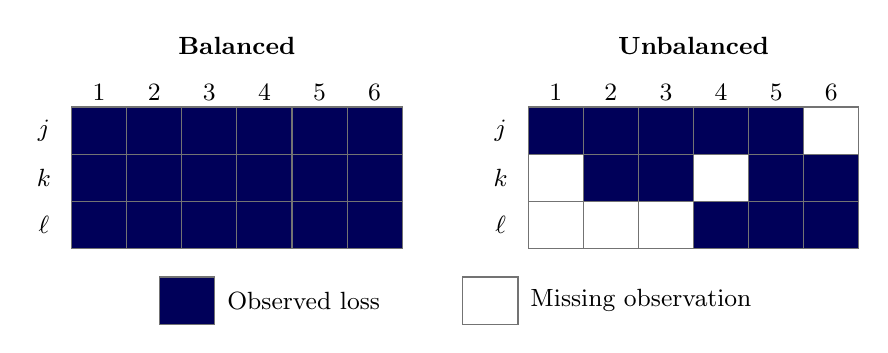
\begin{tikzpicture}[
      x=7mm, y=6mm, font=\small,
      cell/.style={draw=black!55, minimum width=7mm, minimum height=6mm, inner sep=0pt},
      observed/.style={cell, fill=blue!35!black},
      missing/.style={cell, fill=white},
    ]
      \foreach \heading/\offset in {Balanced/0cm, Unbalanced/5.8cm} {
        \begin{scope}[xshift=\offset]
          \node[font=\small\bfseries] at (3.5,1.8) {\heading};
          \foreach \period in {1,...,6} {
            \node at (\period,0.8) {\period};
            \foreach \row in {0,1,2} {
              \node[missing] at (\period,-\row) {};
            }
          }
          \foreach \forecaster/\row in {j/0,k/1,\ell/2} {
            \node at (0,-\row) {$\forecaster$};
          }
        \end{scope}
      }

      \foreach \period in {1,...,6} {
        \foreach \row in {0,1,2} {
          \node[observed] at (\period,-\row) {};
        }
      }
      \begin{scope}[xshift=5.8cm]
        % Observation periods for rows j, k, and ell, respectively.
        \foreach \row/\periods in {0/{1,2,3,4,5}, 1/{2,3,5,6}, 2/{4,5,6}} {
          \foreach \period in \periods {
            \node[observed] at (\period,-\row) {};
          }
        }
      \end{scope}

      \node[observed] at (2.6,-3.6) {};
      \node[right] at (3.15,-3.6) {Observed loss};
      \node[missing] at (8.1,-3.6) {};
      \node[right] at (8.65,-3.6) {Missing observation};
    \end{tikzpicture}
    \caption[Balanced and unbalanced forecast panels]{Balanced and unbalanced forecast
      panels. Rows represent forecasters and columns represent periods. In the balanced
      panel, all three forecasters are observed over the same six periods. In the unbalanced
      panel, $j$ and $k$ share $T_{jk}=\{2,3,5\}$ ($n_{jk}=3$), while $j$ and $\ell$ share
      $T_{j\ell}=\{4,5\}$ ($n_{j\ell}=2$).}
    \label{fig:panel-balance}
  \end{figure}}

\newcommand{\figContrastCovarianceRoutes}{%
  \begin{figure}[!htb]
    \centering
    \begin{tikzpicture}[
      font=\small,
      box/.style={draw=black!55, rounded corners=2pt, align=center, inner sep=3pt},
      route/.style={box, minimum width=6.1cm, minimum height=10.5mm},
      estimate/.style={route, fill=blue!6, minimum height=20mm},
      shared/.style={box, fill=black!5, minimum width=8.5cm},
      line/.style={semithick, draw=black!75},
      link/.style={line, ->},
    ]
      \node[shared] (differences) {\textbf{Pairwise loss differences}\\
        $\dser{jk}_t=X_{t,j}-X_{t,k}$ on $t\in T_{jk}$};

      \node[estimate, below=5mm of differences, xshift=-3.3cm] (mds)
        {\textbf{\MDS{} reconstruction}\\
         Pairwise HAC standard errors $\seNW{jk}$\\
         Double-centre their squares\\
         $\Sigmahat=-\tfrac12 J S^2 J\in\Real^{p\times p}$};
      \node[estimate, below=5mm of differences, xshift=3.3cm] (direct)
        {\textbf{Direct covariance}\\
         Joint HAC on the difference series\\
         Covariance of contrast means\\
         $\Omegahat\in\Real^{q\times q}$};

      \node[route, below=2.5mm of mds] (mdsPSD)
        {Level-space PSD projection, then $A$\\
         $A\Sigmahat^+ A^\top$};
      \node[route, below=2.5mm of direct] (directPSD)
        {Contrast-space PSD projection\\
         $\Omegahat^+$};

      \coordinate[below=2.5mm of differences] (split);
      \coordinate (merge) at ([yshift=-2.5mm]differences.center |- mdsPSD.south);
      \node[shared, below=2.5mm of merge] (simulation)
        {\textbf{Simulate and studentize Gaussian contrasts}\\
         Divide by $\seNW{a}$ (\MDS) or $\sqrt{(\Omegahat^+)_{aa}}$ (direct)};
      \node[shared, below=2.5mm of simulation] (sets)
        {Romano--Wolf stepdown $\;\longrightarrow\;$
         \textbf{Simultaneous rank confidence sets} $\rankci{j}$};

      \draw[line] (differences) -- (split);
      \draw[link] (split) -| (mds);
      \draw[link] (split) -| (direct);
      \draw[link] (mds) -- (mdsPSD);
      \draw[link] (direct) -- (directPSD);
      \draw[line] (mdsPSD.south) |- (merge) -| (directPSD.south);
      \draw[link] (merge) -- (simulation);
      \draw[link] (simulation) -- (sets);
    \end{tikzpicture}
    \caption[Two routes to contrast covariance]{Two routes to contrast covariance.
      The superscript $+$ denotes projection onto the positive semi-definite (PSD) cone.
      The matrix $A$ maps level draws to pairwise contrasts indexed by $a=(j,k)$,
      with $q=\binom{p}{2}$ pairs in the full comparison family.}
    \label{fig:contrast-covariance-routes}
  \end{figure}}

\newcommand{\figMcCrossover}{%
  \begin{figure}[htb]
    \centering
    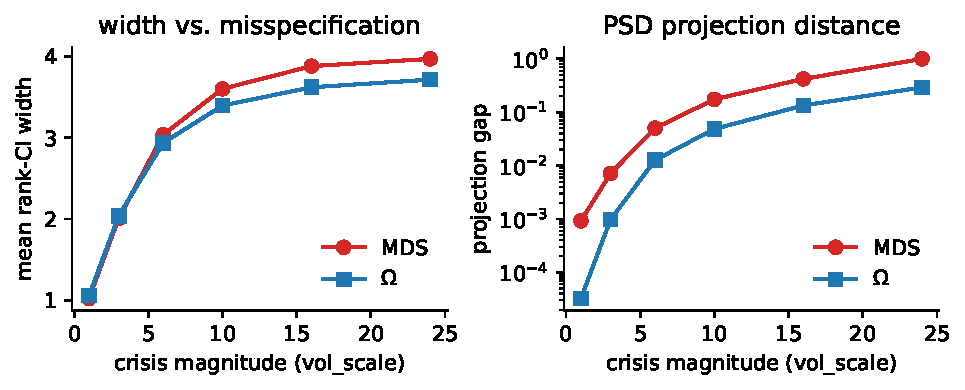
\includegraphics[width=\linewidth]{mc_crossover}
    \caption[Width crossover and projection distance]{Width crossover under growing
      non-stationarity, with imbalance fixed at $0.4$. \emph{Left:} the mean rank-CI
      width of the two constructions as the crisis magnitude grows; the direct
      construction ($\OmegaDirect$) becomes sharper than MDS. \emph{Right:} the MDS
      projection distance grows monotonically, driving the loss of calibration; the
      direct construction's distance, of a different matrix, is shown for reference. $R=500$,
      $B=2000$, $\alpha=0.05$.}
    \label{fig:mc-crossover}
  \end{figure}}

\newcommand{\figGjpCaterpillar}{%
  \begin{figure}[htb]
    \centering
    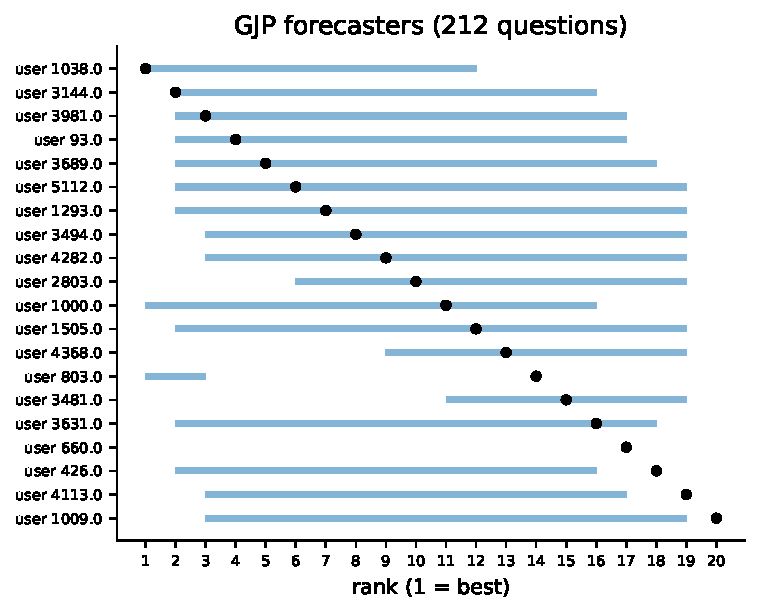
\includegraphics[width=0.72\linewidth]{gjp_caterpillar}
    \caption[GJP rank confidence sets]{Rank confidence sets for the twenty most active
      GJP forecasters (pooled tournament years~1--2, 212 questions, $\alpha=0.2$).
      Bars are the rank sets, dots the point ranks; forecasters are sorted best to
      worst. The best is confidently in the top three, the worst is pinned to last, and
      the middle remains wide --- the partial regime.}
    \label{fig:gjp-caterpillar}
  \end{figure}}

\newcommand{\figMcompCaterpillar}{%
  \begin{figure}[htb]
    \centering
    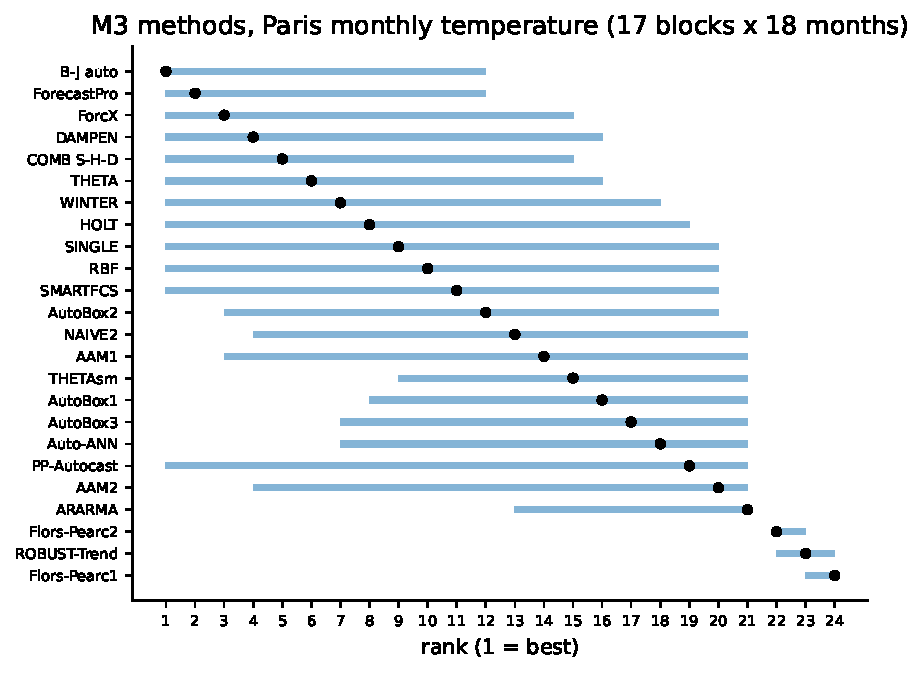
\includegraphics[width=0.75\linewidth]{mcomp_caterpillar}
    \caption[M3 methods on the Paris temperature record]{Rank confidence sets for the 24
      official M3 submissions on the Paris monthly temperature record (17 blocks
      $\times$ 18 held-out months, sMAPE, direct $\OmegaDirect$, $\alpha=0.1$). Bars are
      the rank sets, dots the point ranks. Twelve methods share rank one; three
      systematic failures are pinned to the last three ranks.}
    \label{fig:mcomp-caterpillar}
  \end{figure}}

\newcommand{\figSpfDepErrors}{%
  \begin{figure}[htb]
    \centering
    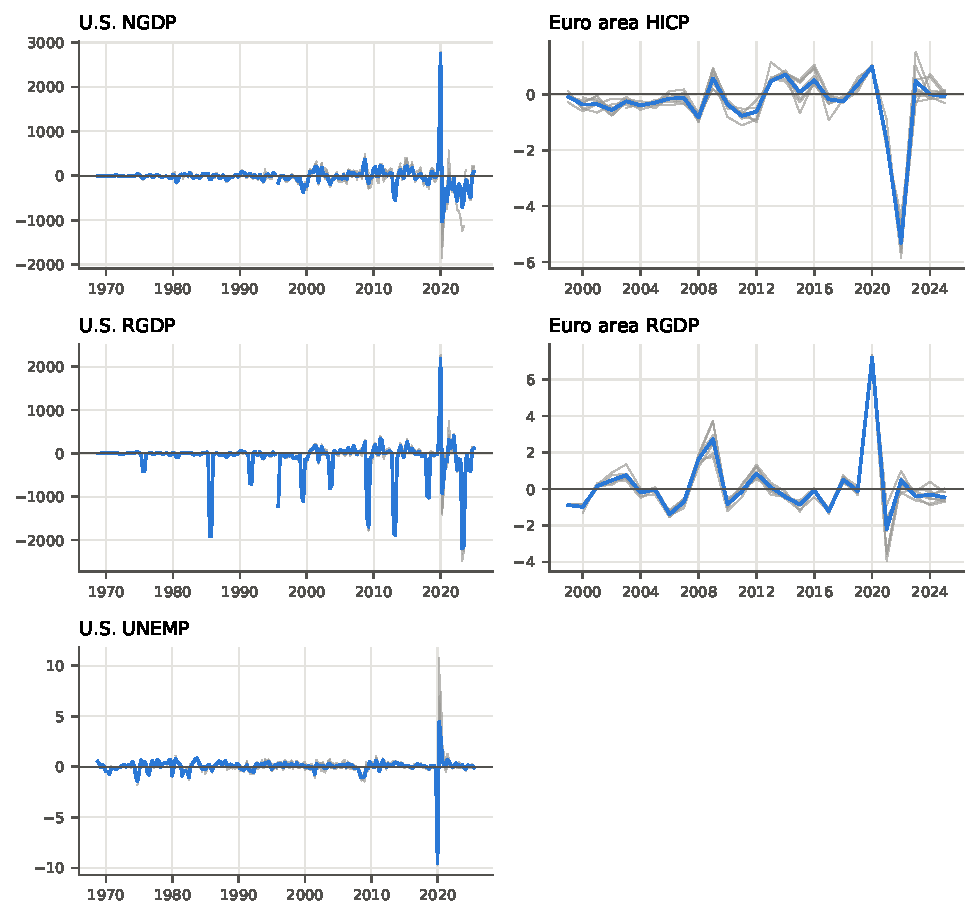
\includegraphics[width=0.9\linewidth]{spf_dep_errors}
    \caption[SPF forecast errors over time]{Forecast errors (forecast minus realization)
      of the eight best-covered forecasters (grey) and the cross-sectional mean of all
      forecasters (blue). Individual errors track the common component closely in every
      panel. The recurrent spikes in U.S.\ RGDP are base-year changes
      (Appendix~\ref{app:spf-dep-rebasing}).}
    \label{fig:spf-dep-errors}
  \end{figure}}

\newcommand{\figSpfDepAcf}{%
  \begin{figure}[htb]
    \centering
    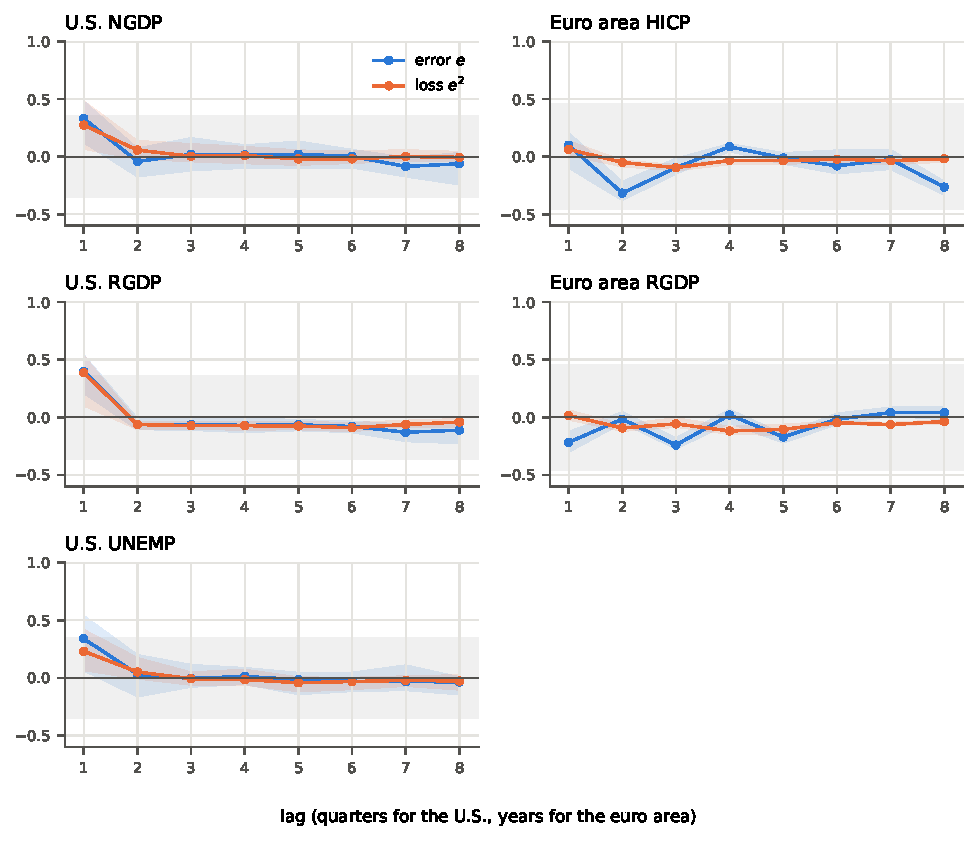
\includegraphics[width=0.9\linewidth]{spf_dep_acf}
    \caption[Autocorrelation of SPF errors and losses]{Autocorrelation of individual
      forecasters' errors $e$ and losses $e^2$: median across forecasters (line) and
      inter-quartile range (shaded). The grey band is the white-noise band
      $\pm1.96/\sqrt{n_1}$ at the median $n_1$.}
    \label{fig:spf-dep-acf}
  \end{figure}}
